
\section{Neural Networks and Deep Learning}
\label{sec:dl}

\subsection{Multi-Layer Perceptrons}
\label{sec:mlp}

The multi-layer perceptron (MLP) is the simplest neural network architecture.
An MLP applies a series of $L$ transformations, typically called \textit{layers}, to an input vector $\mathbf{x} \in \mathbb{R}^{d_{\text{in}}}$ to produce an output vector, not necessarily of the same length.
Each layer $\ell$ consists of an affine transformation followed by a pointwise non-linearity
\begin{equation}
    \mathbf{h}^{(\ell)} = \sigma\!\left( W^{(\ell)} \mathbf{h}^{(\ell-1)} + \mathbf{b}^{(\ell)} \right),
    \label{eqn:mlp_layer}
\end{equation}
where $\mathbf{h}^{(0)} = \mathbf{x}$, $W^{(\ell)} \in \mathbb{R}^{d_\ell \times d_{\ell-1}}$ is the weight matrix, $\mathbf{b}^{(\ell)} \in \mathbb{R}^{d_\ell}$ is the bias vector, and $\sigma$ is an elementwise nonlinear function, called the \textit{activation function}.
The final layer of the network produces the network output, and often either does not have a nonlinearity or has a task-specific one such as a softmax for classification tasks.
The weights and biases $\theta = \{W^{(\ell)}, \mathbf{b}^{(\ell)}\}_{\ell=1}^{L}$, together often referred to simply as the network \textit{weights}, are the learnable parameters of the network.
The traditional diagram of the MLP architecture is shown in \Cref{fig:mlp}.
Here $d_{\text{in}}$ is 10, $L$ is 3, $d_1$ and $d_2$ are both 12, and $d_3$ (the output dimension) is 1.
Note that the circles in the diagram correspond to the hidden states in between the layers of the network.
The lines connecting the circles represent the weight matrices, while the biases and non-linearities are not shown.

\begin{figure}[ht]
    \centering
    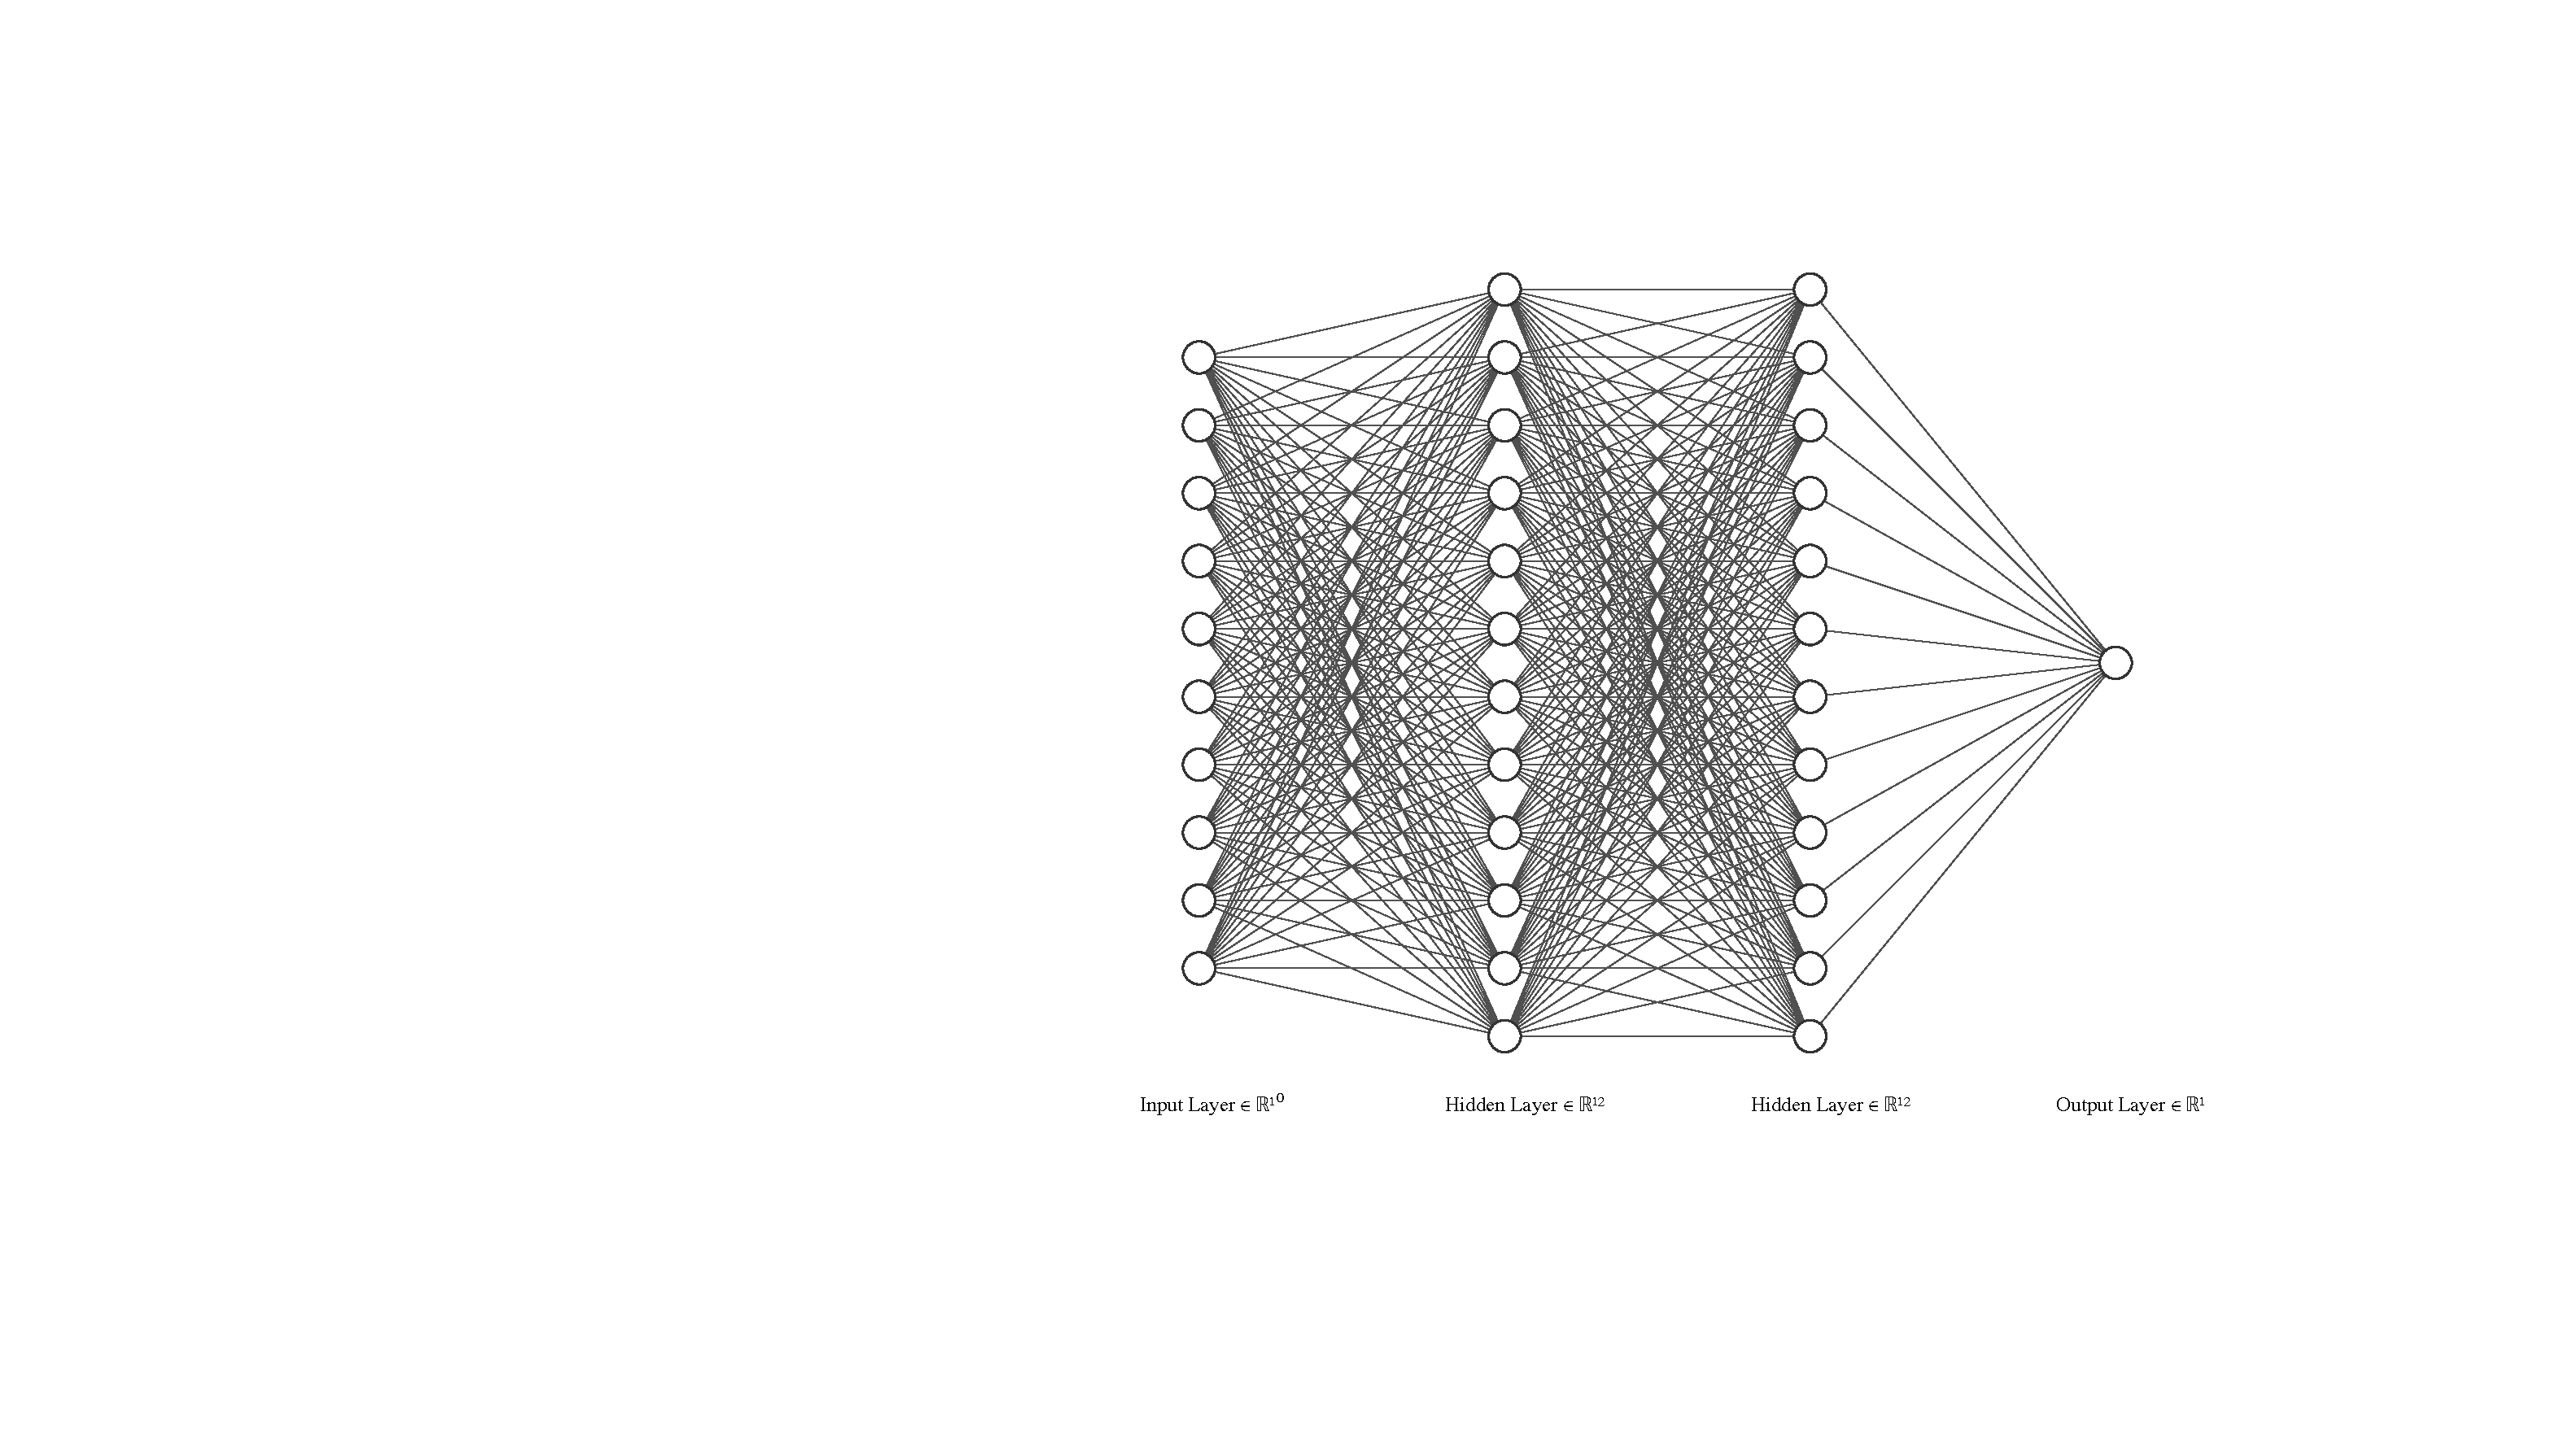
\includegraphics[width=0.75\linewidth, alt={Diagram of a multi-layer perceptron with two hidden layers. Nodes representing input features are shown on the left, connected by arrows to two columns of hidden-layer nodes in the middle, which are in turn fully connected to output nodes on the right.}]{figures/ch3/mlp.pdf}
    \caption{A diagram of a multi-layer perceptron with two hidden layers. In standard MLPs, each node in a given layer is connected to every node in the adjacent layer (fully connected). The input layer receives the feature vector $\mathbf{x}$, and the output layer produces the network's prediction. The circles represent the hidden states in between the layers of the network. The lines connecting the circles represent the weight matrices, while the biases and non-linearities are not shown.}
    \label{fig:mlp}
\end{figure}

In principle the activation function $\sigma$ can be any non-linear function, but in practice the choice can be important for network training.
Examples of activation functions are plotted in \Cref{fig:activations}.
Early networks utilized the sigmoid or hyperbolic tangent activations, but these led to \textit{vanishing gradients} in deep networks where multiplying together gradients taken through multiple activations (see \cref{sec:training}) led to an exponential decay in the magnitude of the gradients at the first hidden layer as the network depth increased.
The \textit{rectified linear unit} (ReLU), defined as $\text{ReLU}(z) = \max(0, z)$, became the standard activation following the AlexNet moment given its gradient is either 0 or 1, meaning no exponential decay.
ReLU activations, however, introduce problems of their own, such as the \textit{dying ReLU problem} where if a neuron's value becomes very negative due to some large gradient early in training its gradients are zeroed throughout the rest of training.
ReLU-based MLPs also have a zero second derivative, which can be limiting in specific applications and prohibit the use of second-order optimizers.
Recently smoother non-linearities have become common.
The most important one is the \textit{Gaussian error linear unit} (GELU), defined as $\text{GELU}(z) = z \cdot \Phi(z)$ where $\Phi$ is the standard normal CDF.
GELU has become the preferred activation in many modern architectures, including the transformer networks used in \cref{ch:zjets}.
These functions are plotted in \Cref{fig:activations}.

\begin{figure}[ht]
    \centering
    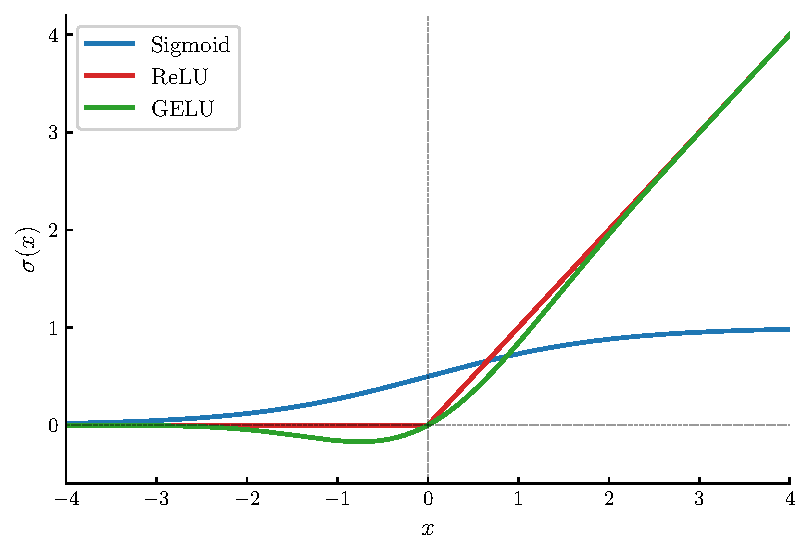
\includegraphics[width=0.7\linewidth, alt={Line plots of the ReLU and GELU activation functions. ReLU is zero for negative inputs and linear for positive inputs, with a sharp corner at the origin. GELU is similar but smoothly curved near zero, with a slight negative dip for small negative inputs.}]{figures/ch3/activation_functions.pdf}
    \caption{The ReLU and GELU functions commonly used as activations in modern neural networks, plotted against the input $x$.}
    \label{fig:activations}
\end{figure}

The most important property of MLPs is that they are universal function approximators, meaning that an MLP with a single hidden layer of sufficient width can approximate any continuous function on a compact domain to arbitrary precision~\cite{cybenko1989approximation,hornik1989multilayer}.
The MLP is in principle flexible enough to approximate any function, even for example the very complicated functions contained in modern LLMs.
In practice this property of MLPs is of limited use because it guarantees only that a solution exists, not that it can be found by any of the gradient-based optimization strategies discussed below.
Deep MLPs and more sophisticated network architectures are used much more widely than very wide, two-layer MLPs because they are empirically observed to find much better solutions when trained with gradient descent.
There are some theoretical motivations for why this might be the case~\cite{jacot2018neural}, but there is not a rigorous theory explaining why some networks optimize better than others.
The MLP architecture on its own is little used in modern deep learning, but it is used as a component in graph and transformer architectures.

\subsection{Training Neural Networks}
\label{sec:training}

The task of training a neural network is to find parameter values $\theta$ that minimize a scalar loss function $\mathcal{L}(\theta)$ computed over a training dataset.
The canonical example of a loss function is the binary cross-entropy (BCE) loss used for binary classification tasks with inputs $\mathbf{x}_i$ and labels $y_i \in \{0, 1\}$,
\begin{equation}
    \mathcal{L}_{\text{BCE}}(\theta) = -\frac{1}{N} \sum_{i=1}^{N} \left[ y_i \log f_\theta(\mathbf{x}_i) + (1 - y_i) \log\!\left(1 - f_\theta(\mathbf{x}_i)\right) \right],
    \label{eqn:bce}
\end{equation}
where $f_\theta(\mathbf{x}_i) \in (0,1)$ is the network's predicted probability that example $i$ belongs to class 1.
Minimizing the BCE loss is equivalent to maximizing the log-likelihood of the training data under the assumption that their labels are described by a Bernoulli random variable.
Constructing loss functions that maximize the log-likelihood of the training data is a recurring pattern across machine learning.

\subsubsection{Backpropagation}

Most supervised and unsupervised machine learning methods approach minimizing $\mathcal{L}(\theta)$ by computing its gradient with respect to each parameter of the model.
The \textit{backpropagation} algorithm allows for the calculation of gradients for each parameter in a deep network by applying the chain rule of calculus layer by layer.
Concretely, the pre-activation neuron value at layer $\ell$ is $\mathbf{z}^{(\ell)} = W^{(\ell)} \mathbf{h}^{(\ell-1)} + \mathbf{b}^{(\ell)}$.
Application of the activation yields the neuron value $\mathbf{h}^{(\ell)} = \sigma(\mathbf{z}^{(\ell)})$.
Gradients must be computed for both the weights and biases of layer $\ell$.
First, the gradient of the loss with respect to the weights of layer $\ell$ is
\begin{equation}
    \frac{\partial \mathcal{L}}{\partial W^{(\ell)}} = \boldsymbol{\delta}^{(\ell)} \left(\mathbf{h}^{(\ell-1)}\right)^\top,
    \label{eqn:backprop_W}
\end{equation}
where the error signal $\boldsymbol{\delta}^{(\ell)}$ is defined recursively as
\begin{equation}
    \boldsymbol{\delta}^{(\ell)} = \left( \left(W^{(\ell+1)}\right)^\top \boldsymbol{\delta}^{(\ell+1)} \right) \odot \sigma'\!\left(\mathbf{z}^{(\ell)}\right),
    \label{eqn:backprop_delta}
\end{equation}
with $\boldsymbol{\delta}^{(L)}$ initialized from the derivative of the loss with respect to the network output and $\odot$ denoting elementwise multiplication.
Starting with $\ell = L$, $\boldsymbol{\delta}^{(\ell)}$ can be computed and then used as the starting point for the calculation of gradients at layer $\ell = L - 1$.
This process was implemented in software for early deep learning frameworks such as Theano, and later TensorFlow 1.x.
All modern deep learning frameworks (PyTorch, JAX, TensorFlow) implement automatic differentiation, which computes gradients through arbitrary compositions of differentiable tensor operations without the user needing to implement \Cref{eqn:backprop_W,eqn:backprop_delta} explicitly.\footnote{The three major frameworks differ in how they implement automatic differentiation. TensorFlow 1.x and Theano used \textit{static computation graphs} where the full computational graph is defined and compiled before any data is processed. PyTorch and TensorFlow 2.x use \textit{dynamic computation graphs} (define-by-run), where the graph is constructed on the fly during the forward pass. JAX makes automatic differentiation as a first-class function transformation (\texttt{jax.grad}) that can be composed with other transforms such as vectorization (\texttt{jax.vmap}) and JIT compilation (\texttt{jax.jit}).}

\subsubsection{Gradient Descent and Optimization}

Once gradients of the loss with respect to all network parameters have been calculated, the parameters can be updated by gradient descent:
\begin{equation}
    \theta \leftarrow \theta - \eta \, \nabla_\theta \mathcal{L}(\theta),
    \label{eqn:gd}
\end{equation}
where $\eta > 0$ is the learning rate.
Intuitively, the negative gradient points in the direction of steepest descent on the loss surface, visualized in two dimensions in \Cref{fig:gradient_descent}.
Each update steps the parameters in the direction that minimizes the loss.
This simple procedure is effective but has limitations.
It has no guarantees about convergence to the global minimum.
Optimization can get stuck in local minima, and also depend strongly on the random initialization of the network weights and biases.
This effect is illustrated in \Cref{fig:gradient_descent}, where the red path converges to a local minimum while the orange path converges to the true global minimum.
The paths differ only by the initialization of the two parameters $\theta_1$ and $\theta_2$. 
Note however that these limitations can matter much less in practice as the fraction of critical points that are minima becomes vanishingly small as the dimensionality of the optimization increases.
This is one of the theoretical explanations for why large neural networks are easier to optimize than small ones.

\begin{figure}[ht]
    \centering
    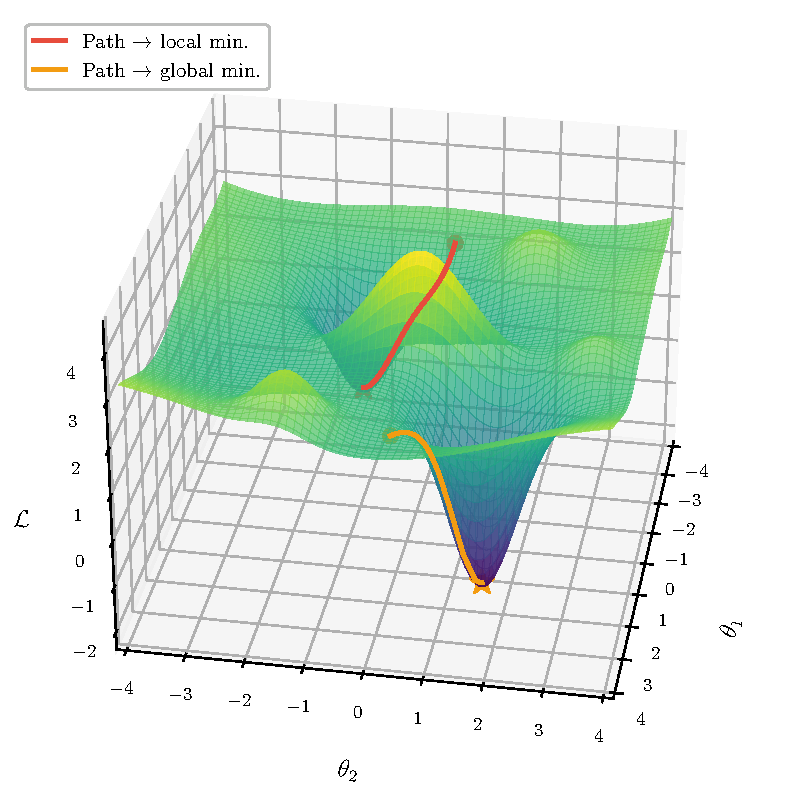
\includegraphics[width=0.65\linewidth, alt={Three-dimensional surface plot of a bowl-shaped loss function over a two-dimensional parameter space. A sequence of points connected by arrows traces a path descending from a high-loss starting point down the surface toward the minimum at the bottom of the bowl.}]{figures/ch3/gradient_descent.pdf}
    \caption{Geometric intuition for gradient descent on a two-dimensional loss surface. Starting from an initial parameter configuration, each update moves in the direction of steepest descent, converging toward a minimum. Gradient descent does not guarantee convergence to the true global minimum. The optimization can depend strongly on the random initialization of the network weights and biases as illustrated by the red and orange paths converging to different minima.}
    \label{fig:gradient_descent}
\end{figure}

In \Cref{eqn:gd}, the loss is computed over the full dataset before gradients are computed.
This requires running a forward and backward pass over the network for each data point in the training set before making a single parameter update, which is computationally inefficient and intractable for large datasets.
\textit{Stochastic gradient descent} (SGD) replaces the losses and gradient calculation over the full dataset with the same calculation over a randomly sampled \textit{mini-batch} of $B$ examples.
This procedure dramatically reduces the per-parameter-update computational cost, but introduces variance into the gradient estimates.
Empirically this variance often aids generalization of trained networks.
The learning rate $\eta$ (followed by the batch size $B$) is usually the most critical hyperparameter for any neural network training.
In modern practice, a \textit{learning rate scheduler} that adjusts $\eta$ over the course of training is typically applied.

In SGD, a single learning rate is used for each parameter in a network.
A more advanced alternative is \textit{adaptive optimizers}, which maintain per-parameter estimates of gradient statistics over the past few mini-batches, and adjust the learning rate per parameter based on the size of past gradients.
The commonly used Adam optimizer~\cite{kingma2014adam} computes exponential moving averages of the gradient $m_t$ and the squared gradient $v_t$:
\begin{align}
    m_t &= \beta_1 m_{t-1} + (1 - \beta_1) g_t, \label{eqn:adam_m} \\
    v_t &= \beta_2 v_{t-1} + (1 - \beta_2) g_t^2, \label{eqn:adam_v}
\end{align}
where $g_t = \nabla_\theta \mathcal{L}$ is the gradient at step $t$ and $\beta_1, \beta_2 \in (0,1)$ are decay rates.
Bias-corrected estimates $\hat{m}_t = m_t / (1 - \beta_1^t)$ and $\hat{v}_t = v_t / (1-\beta_2^t)$ are used to compute the parameter update $\theta \leftarrow \theta - \eta \, \hat{m}_t / (\sqrt{\hat{v}_t} + \epsilon)$.
The intuition is that parameters with consistently large (small) gradients receive smaller (larger) updates due to the factor of $\sqrt{v_t}$ in the denominator, allowing networks with a large range of gradient scales to be trained efficiently.

\subsubsection{Generalization and Regularization}

A trained model may not perform well on unseen data if it has ``memorized'' the specific data points rather than learning the underlying function.
This is called \textit{overfitting}, and is best understood as one extreme of the \textit{bias--variance tradeoff}.
A model with low capacity will be unable to fit the training data (high bias) and will simply predict a best guess for all data points (low variance).
A model with high capacity is able to memorize specific training examples (low bias), but can overfit to the data and yield very different results for only slightly different inputs (high variance).
\Cref{fig:bias_variance} illustrates overfitting and the bias--variance tradeoff in a 1D regression problem solved with a polynomial fit.
A model with too little capacity (e.g. too few polynomial degrees) underfits and has high bias, while a model with too much capacity (e.g. too many polynomial degrees) that is not properly regularized overfits and has high variance.

\begin{figure}[t]
    \centering
    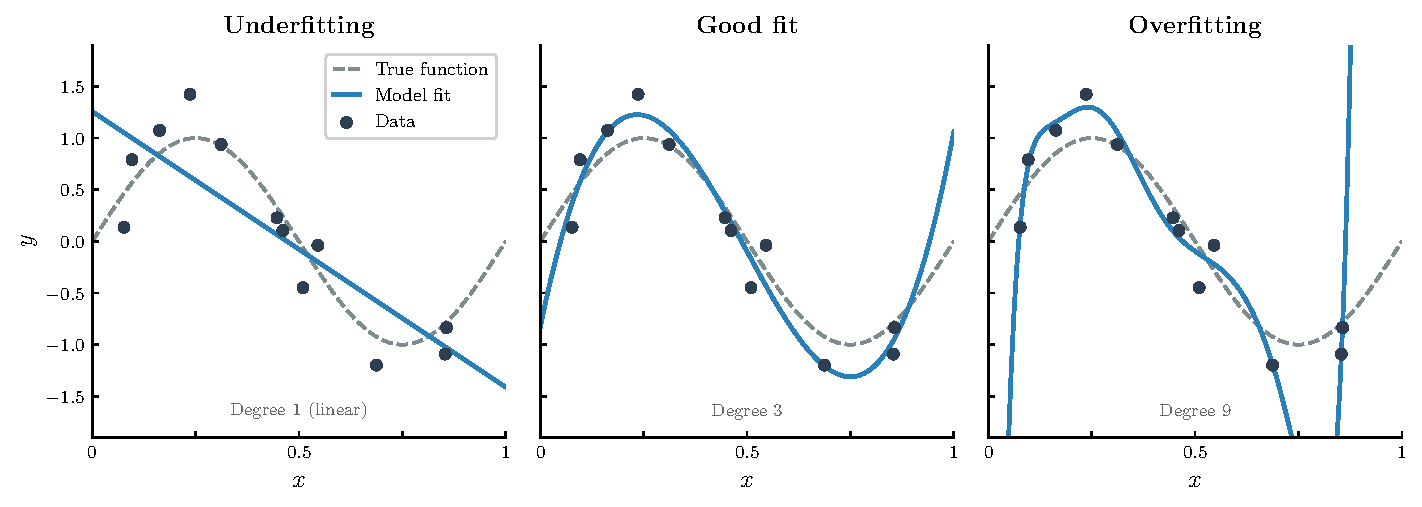
\includegraphics[width=0.8\linewidth, alt={Three scatter plots with fitted curves illustrating the bias--variance tradeoff. The left plot shows an underfit model with a straight line that misses the curved trend in the data (high bias). The center plot shows a well-fit smooth curve that captures the underlying trend. The right plot shows an overfit model with a highly wiggly curve that passes through noise (high variance).}]{figures/ch3/bias_variance.pdf}
    \caption{Illustration of the bias--variance tradeoff in the context of a 1D regression problem fitting a polynomial model. An underfit model with one polynomial degree (left) has high bias and fails to capture the true structure in the data. An overfit model with many polynomial degrees (right) has high variance and memorizes noise rather than the underlying function. The goal is to find the intermediate regime (center) that generalizes well.}
    \label{fig:bias_variance}
\end{figure}

\textit{Generalization} is a model's ability to produce accurate predictions on unseen data.
Standard practice to ensure generalization is to partition available data into three disjoint subsets: a \textit{training set} used to train the model, a \textit{validation set} used to monitor performance on held-out data during training, and a \textit{test set} used for a single final evaluation after training is complete.
Gradients are never computed using the validation or test sets.
A classic signal of overfitting is when the loss, calculated over the validation set, begins to decrease with further training, while the training loss always decreases since it is directly minimized.
\textit{Regularization} is a set of methods for preventing the model from overfitting.
A simple regularization strategy is early stopping, in which training is terminated when the validation loss stops decreasing, preventing the network from entering the high variance overfitting regime.
\Cref{fig:early_stopping} shows a typical training curve illustrating this procedure.
The training loss (blue curve) decreases monotonically except for small noise caused by the stochastic gradient estimates computed on mini-batches.
The validation loss (red curve) follows the training loss initially before flattening out and beginning to increase as the model overfits.
The configuration of model weights that offers the best generalization (lowest validation loss) is marked in the Figure.
In early stopping, training is stopped after the validation loss fails to decrease for some number of epochs, called the \textit{patience}, to account for the noise in the validation loss.\footnote{The relationship between model capacity, dataset size, and generalization in modern overparameterized networks with many more parameters than training examples is more subtle than the usual bias--variance tradeoff picture. Very large models that are trained well past the point of interpolating the training data sometimes exhibit \textit{double descent}: a second regime in which increasing capacity or training time actually improves generalization.}

\begin{figure}[t]
    \centering
    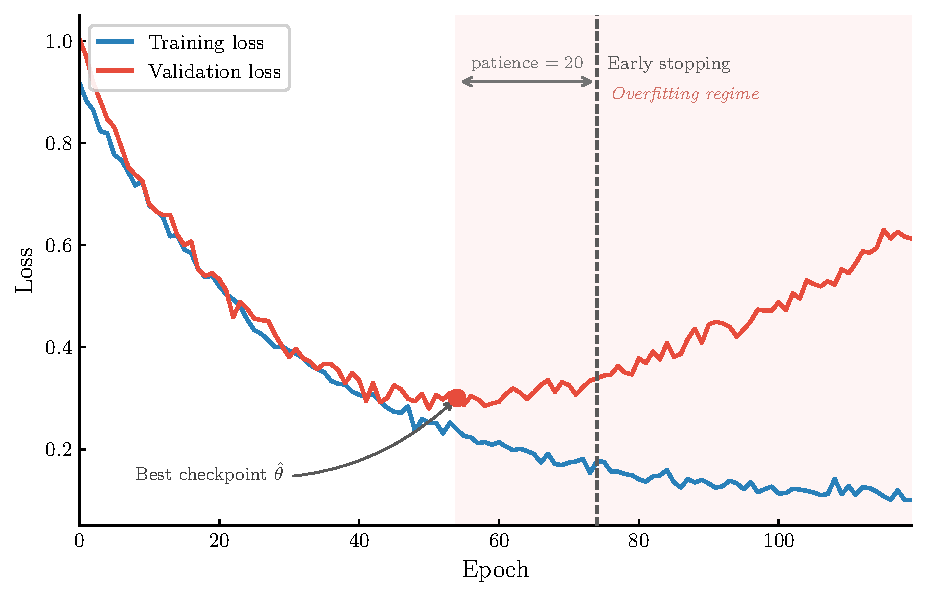
\includegraphics[width=0.7\linewidth, alt={Line plot showing training loss and validation loss as a function of training epoch. The training loss decreases monotonically. The validation loss decreases initially then rises after reaching a minimum. A vertical dashed line marks the epoch of minimum validation loss, labeled as the early stopping point.}]{figures/ch3/early_stopping.pdf}
    \caption{Training and validation loss curves illustrating early stopping. The training loss is plotted in blue and the validation loss in red. The configuration of model parameters that minimizes the validation loss is marked. Training past this point results in sub-optimal generalization. Early stopping with a patience of 20 epochs is marked by the vertical dashed line, indicating where model training would be stopped.}
    \label{fig:early_stopping}
\end{figure}

Two other widely used regularization techniques are \textit{dropout} and \textit{weight decay}.
Dropout~\cite{hinton2012improving} randomly zeros a set of activation functions with probability $p$, called the \textit{dropout probability}, during training.
At inference time, all activations are retained.
Weight decay adds an L2 norm penalty on the parameters of the network $\|\theta\|^2$ to the loss.
This discourages large weights and limits the capacity of the network to overfit.
Weight decay can be understood as placing a zero-mean Gaussian prior on the network parameters.

\subsection{Convolutional Neural Networks}
\label{sec:cnn}

MLPs operate on flat vectors of inputs and have no \textit{implicit bias}, or architectural specialization to a given known structure in the input data.
Convolutional neural networks (CNNs) encode \textit{translational symmetry} into the network architecture, meaning that a feature at one spatial location should not affect the network output if shifted to another location.
This is achieved by \textit{weight sharing}, in which a set of weights and biases, often called a \textit{filter}, is scanned across the inputs rather than applying a separate set of weights per position.
CNNs were first developed for computer vision tasks using image data as input.
Specifically AlexNet was an early example of a CNN architecture.

Concretely, a CNN layer applies a set of $F$ learned filters $\{k_f\}_{f=1}^F$.
The set of learned weights that define each filter are often called a \textit{kernel}.
The kernel has a spatial extent $K$ (or $K \times K$ for 2D convolutions) which gives the number of input positions it considers at one time, and a depth which is equal to the number of \textit{channels} attached to each input position $C_{\text{in}}$.
The number of output channels is equal to the number of filters $F = C_{\text{out}}$.
For the specific case of a 2D convolution, the output at spatial position $(i, j)$ and output channel $f$ is
\begin{equation}
    h_{f,i,j} = \sigma\!\left( \sum_{c=1}^{C_{\text{in}}} \sum_{p=0}^{K-1} \sum_{q=0}^{K-1} k_{f,c,p,q} \cdot x_{c,\, i+p,\, j+q} + b_f \right),
    \label{eqn:conv2d}
\end{equation}
where $x_{c,i,j}$ is the input at channel $c$ and position $(i,j)$, $k_{f,c,p,q}$ are the kernel weights, and $b_f$ is the kernel bias.
The number of channels $C$ sets how many floating point numbers are used to represent each spatial location.
For the input layer in image data this is typically 3 (RGB color channels), but it grows to hundreds in the deeper layers of large networks.
This channel dimension is also directly analogous to the \textit{hidden dimension} of transformer models, which will be discussed in \Cref{sec:attention} and used extensively in this thesis.
The filters of a given convolutional layer are sometimes applied with a \textit{stride} $s > 1$, meaning they advance by $s$ positions at each step.
This makes the number of spatial sites in the output smaller than in the input, allowing the network to extract increasingly broad summary features.

Another important operation in CNNs is \textit{pooling}, in which an aggregation operation like maximum (\textit{max pooling}) or average (\textit{average pooling}) is applied across a spatial region.
As with setting a filter's stride to be greater than one, pooling reduces the spatial dimensions of feature maps and encourages the network to extract broader summary features as depth increases.
Both operations are illustrated in \Cref{fig:convolution}.

\begin{figure}[htbp]
    \centering
    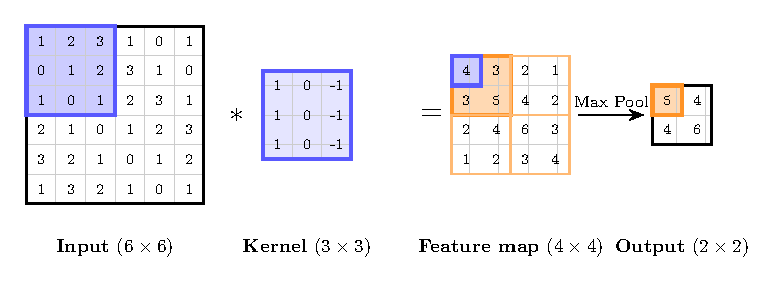
\includegraphics[width=0.85\linewidth, alt={Two-part diagram illustrating CNN operations. On the left, a 2D convolution is shown: a small learned filter slides over an input feature map and computes dot products at each position to produce a smaller output feature map. On the right, max pooling is shown: the feature map is divided into non-overlapping regions and the maximum value in each region is retained, reducing the spatial dimensions by a factor of two.}]{figures/ch3/convolution_diagram}
    \caption{The two core spatial operations in a convolutional neural network. \textit{Left}: a learned $K \times K$ kernel is convolved with the input feature map to produce a new feature map, with each output value capturing local spatial structure. \textit{Right}: max pooling partitions the feature map into non-overlapping windows and retains only the maximum activation in each, reducing spatial resolution and providing local translation invariance.}
    \label{fig:convolution}
\end{figure}

Just like with MLPs, very deep CNNs were found to suffer from vanishing gradients.
One method developed to address this was the \textit{residual} or \textit{skip} connection~\cite{He:2015resnet}, in which the output of a set of operations is added to its input:
\begin{equation}
    \mathbf{h}_{\text{out}} = \mathcal{F}(\mathbf{h}_{\text{in}}) + \mathbf{h}_{\text{in}},
    \label{eqn:residual}
\end{equation}
where $\mathcal{F}$ denotes one or more operations\footnote{Re-arranging this equation implies that the role of the operations is to learn \textit{residual} corrections on the data representation needed to minimize the loss. This idea connects to the idea of \textit{boosting} in tree models and to the diffusion models introduced in \Cref{sec:diffusion}.}.
The skip connection creates a direct gradient path from the output to the input of each block, making it possible to train networks with hundreds of layers.
The structure of a single residual block is shown in \Cref{fig:resblock}.

\begin{figure}[ht]
    \centering
    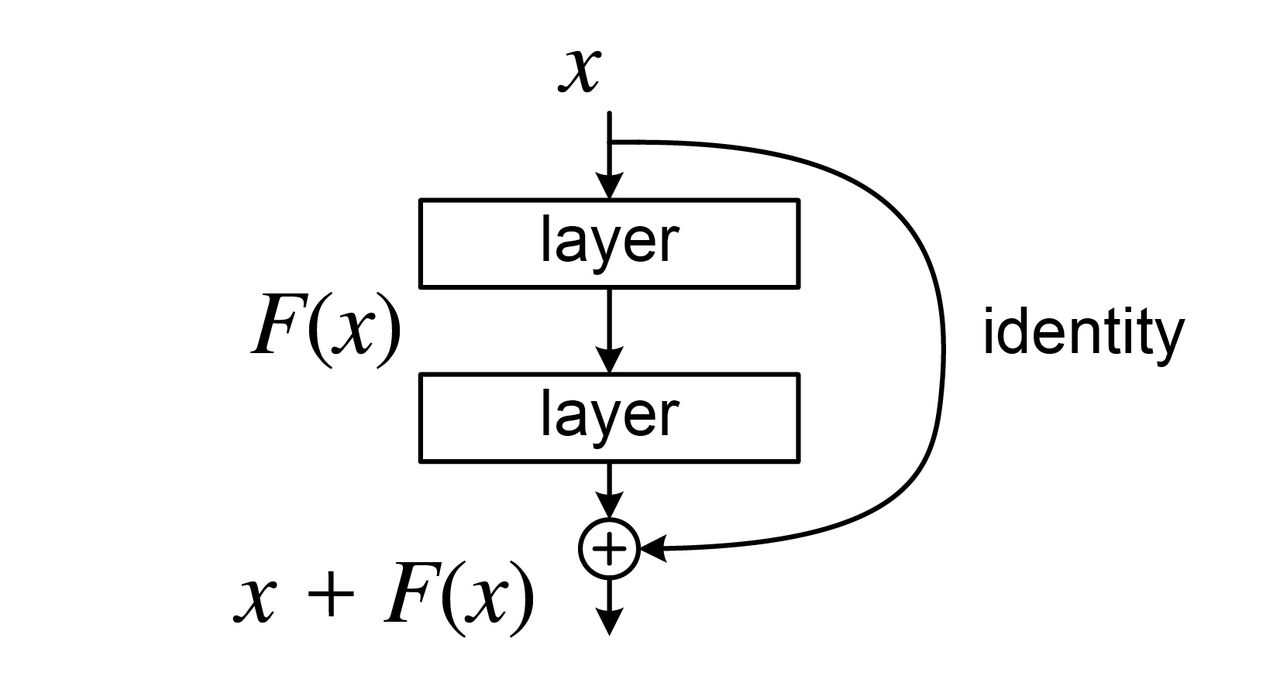
\includegraphics[width=0.35\linewidth, alt={Diagram of a residual block. An input arrow enters from the top and splits into two paths: one passes through two convolutional layers with a ReLU activation in between, and the other bypasses these layers via a skip connection. The two paths are recombined by addition before a final ReLU activation produces the block output.}]{figures/ch3/ResBlock.png}
    \caption{A single residual block. The block applies two layers of operations (convolution or otherwise) to its input and adds the result to the original input via a skip connection. This design allows gradient signals to propagate cleanly through very deep networks.}
    \label{fig:resblock}
\end{figure}

The \textit{ResNet} architecture~\cite{He:2015resnet} stacks many residual blocks on top of each other as shown in \Cref{fig:resnet}.
The ``ID blocks'' shown in the Figure correspond to skip connections.
ResNet was the dominant image classification architecture for several years after it was introduced in 2015.
The first application of CNNs in HEP was for jet tagging tasks as discussed in \Cref{ch:tagging}, where the energy deposits in a calorimeter were interpreted as a 2D image and used as input to CNN models~\cite{Cogan:2014oua,deOliveira:2017pjk}.
ResNet-based models showed nearly state-of-the-art performance on jet classification tasks as recently as 2019~\cite{Kasieczka:2019dbj}.
They were ultimately superseded by graph neural networks and then transformers, but CNNs are an important part of the history of deep learning applications in HEP.

\begin{figure}[ht]
    \centering
    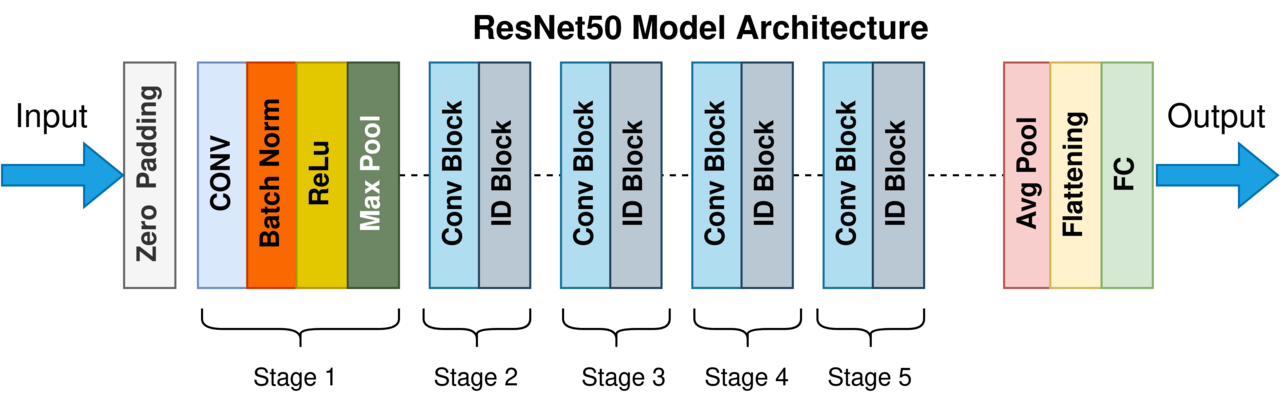
\includegraphics[width=0.9\linewidth, alt={Diagram of the full ResNet architecture. An input image enters a convolutional layer followed by batch normalization and ReLU, then passes through four groups of stacked residual blocks with increasing numbers of output channels and decreasing spatial resolution. The final feature map is globally average-pooled and passed to a fully connected layer that produces class scores.}]{figures/ch3/resnet.png}
    \caption{The ResNet architecture, composed of stacked residual blocks which alternate convolution operations and identity blocks (skip connections). The ResNets in the original paper had hundreds of layers and tens of millions of parameters, which were extraordinarily large in late 2015. Reproduced from \citet{gorlapraveen123_resnet50_2021} via Wikimedia Commons under a \href{https://creativecommons.org/licenses/by-sa/4.0/}{CC~BY-SA~4.0} license.}
    \label{fig:resnet}
\end{figure}

\subsection{Graph Neural Networks}
\label{sec:gnn}

After CNNs, the next major step in the history of deep learning in HEP was to interpret jets as \textit{point clouds} rather than images.
A point cloud is an unordered set of points in a high-dimensional space, for example the four-momenta of the particles in a jet.
Graph neural networks (GNNs)~\cite{Battaglia:2018mnb} interpret sets as graphs, in which each item in the set is a node connected to other nodes in the set by edges.

Most GNNs used in HEP are instances of the \textit{message-passing} framework, where the nodes of an input graph are updated by a series of operations which aggregate \textit{messages} passed along all of the node's edges.
The update at node $i$ after one message-passing step is
\begin{equation}
    \mathbf{h}_i' = \phi_{\text{node}}\!\left( \mathbf{h}_i,\; \bigoplus_{j \in \mathcal{N}(i)} \phi_{\text{edge}}(\mathbf{h}_i, \mathbf{h}_j) \right),
    \label{eqn:message_passing}
\end{equation}
where $\mathbf{h}_i$ is the current feature vector of node $i$, $\mathcal{N}(i)$ is the set of nodes connected to node $i$, $\phi_{\text{edge}}$ is a learned edge function that computes a message from each neighbor, $\bigoplus$ is a permutation-invariant aggregation (e.g.\ sum or max), and $\phi_{\text{node}}$ is a learned update function.
Both $\phi_{\text{edge}}$ and $\phi_{\text{node}}$ are typically implemented as MLPs.

The ParticleNet architecture~\cite{Qu:2019gqs}, which will be applied to a jet classification task in \Cref{ch:tagging}, uses a specific message-passing operation called \textit{edge convolution} (EdgeConv).
In EdgeConv, the message passed along the edge from node $j$ to node $i$ is computed from both the absolute feature of node $j$ and the \textit{relative} feature between $j$ and $i$:
\begin{equation}
    \mathbf{h}_i' = \frac{1}{|\mathcal{N}(i)|} \sum_{j \in \mathcal{N}(i)} \phi_{\text{edge}}\!\left( \mathbf{h}_i,\; \mathbf{h}_j - \mathbf{h}_i \right),
    \label{eqn:edgeconv}
\end{equation}
where $\phi_{\text{edge}}$ is a small MLP.
The relative features $\mathbf{h}_j - \mathbf{h}_i$ capture pairwise distances between inputs and are empirically found to be very useful in HEP, for example because the difference between two particles' four-momenta is physically meaningful.

Another important type of message passing GNN is graph attention networks (GATs), which generalize this pattern by replacing the uniform averaging in \Cref{eqn:edgeconv} with learned, input-dependent weights over the neighborhood.
This is identical to the attention mechanism covered in \Cref{sec:attention}, except with some entries of the attention matrix zeroed such that only inputs within a connected neighborhood of each other can attend.
The better expressivity and better scaling properties of full attention, in which the strength of the connection between two inputs is allowed to be a learned feature, has led attention-based networks to largely supplant GNNs in HEP applications.

\subsection{Attention and Transformers}
\label{sec:attention}

The attention mechanism, and the transformer architecture built on top of it, underlie most consumer AI products in use today.
They have seen equally broad adoption in HEP, so this Section will introduce them in some detail.

The origins of attention were in augmenting recurrent neural networks (RNNs) to perform better on machine translation tasks~\cite{bahdanau2014neural, luong2015effective, cheng2016long, lin2017structured}.
In early versions of attention the decoder of an RNN, whose job is to generate the next output token given the network's current internal representation, could selectively weight all positions in the input sequence according to their relevance to the current decoding step.
This was found to be more performant than compressing every token in the input into a fixed-size vector to provide context for the decoder.
The next conceptual step was to remove the recurrence entirely and simply compute attention between all items in the input sequence, with the relative positions of the items provided to the attention mechanism as positional encodings.
This was the contribution of the famous ``Attention Is All You Need'' paper~\cite{Vaswani:2017attention}\footnote{Arguably the citation count of this paper relative to the initial papers that actually introduced attention is evidence of the Matthew effect in science, in which papers with high citation counts attract even more citations as time goes on. The Vaswani paper became the point of reference for early transformer models like BERT and GPT. That made it the starting point for anyone learning about attention and ensured it would keep being cited in the future. Despite this success Vaswani et al. did not actually invent attention; that credit belongs to Bahdanau et al. and Luong et al.}.
This self-attention operation, without any additional recurrent operations computed on the input sequence, is the backbone of the transformer architecture applied at many points in this thesis and so is worth covering in detail.

The first step of self-attention is to compute three linear projections of the input set.
The input is represented as set of $N$ vectors, each with dimension $d$ and arranged as a matrix $X \in \mathbb{R}^{N \times d}$.
The linear projections are:
\begin{equation}
    Q = X W_Q, \quad K = X W_K, \quad V = X W_V,
    \label{eqn:qkv}
\end{equation}
where $W_Q, W_K, W_V \in \mathbb{R}^{d \times d_k}$ are learned weight matrices, producing three matrices known as the queries $Q$, keys $K$, and values $V$.
$d_k$ is the \textit{key dimension} and is typically set to a small value (e.g. 64) to reduce the computational cost of the attention operation.
Self-attention is then computed using these three matrices as
\begin{equation}
    \text{Attention}(Q, K, V) = \text{softmax}\!\left( \frac{Q K^\top}{\sqrt{d_k}} \right) V.
    \label{eqn:attention}
\end{equation}
The matrix $Q K^\top / \sqrt{d_k} \in \mathbb{R}^{N \times N}$ is the \textit{attention matrix}.
The $(i,j)$-th entry of this matrix can be interpreted as setting how much the input at position $i$ (query) should affect the item at position $j$ (key).
Applying a softmax row-wise ensures that these attention weights for a given query sum to one.
Multiplying by $V$ produces a weighted sum of value vectors for each position, which is the output of the attention operation.
Note that the vectors which determine the attention weights (keys) are not the same as the vectors which are being attended to (values).
This is a key difference between the modern, scaled dot-product attention operation and the original attention operation~\cite{bahdanau2014neural}.
The $\sqrt{d_k}$ scaling factor exists to prevent the variance of the entries of the attention matrix from growing with $d_k$.
Without this factor, the standard deviation of the entries of the pre-softmax attention matrix would grow with the square-root of $d_k$, meaning larger $d_k$ would imply different post-softmax statistics.

In modern practice the self-attention operation is typically applied several times in parallel across $H$ independent \textit{attention heads}, each with its own projection matrices and a smaller key dimension $d_k = d / H$.
Outputs of the heads get concatenated together and finally projected back to dimension $d$:
\begin{equation}
    \text{MultiHead}(Q, K, V) = \text{Concat}(\text{head}_1, \ldots, \text{head}_H) \, W_O,
    \label{eqn:multihead}
\end{equation}
where $\text{head}_h = \text{Attention}(X W_{Q,h}, X W_{K,h}, X W_{V,h})$ and $W_O \in \mathbb{R}^{d \times d}$ is a learned output projection.
The benefit of multi-head attention is that the network can attend to inputs based on different aspects of the relationships between elements.
A diagram of the entire multi-head attention operation is shown in \Cref{fig:multihead_attention}.

\begin{figure}[t]
    \centering
    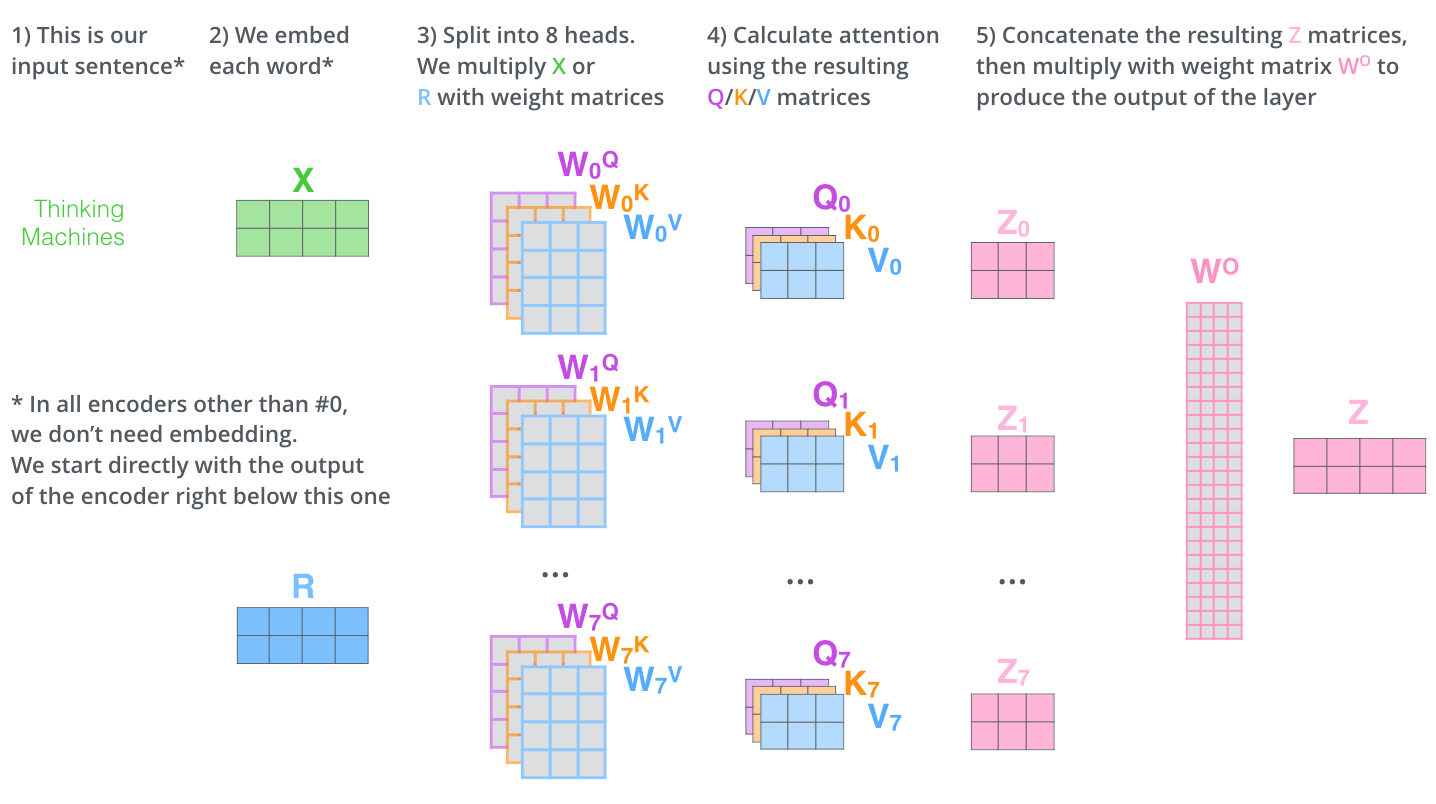
\includegraphics[width=0.85\linewidth, alt={Diagram of scaled dot-product attention and multi-head attention. On the left, the single-head attention mechanism shows queries, keys, and values fed through a matrix multiply, scale, softmax, and final matrix multiply. On the right, the multi-head variant shows H parallel attention heads whose outputs are concatenated and linearly projected.}]{figures/ch3/self-attention-recap}
    \caption{Scaled dot-product attention (left) and multi-head attention (right). Multi-head attention runs $H$ independent attention heads in parallel, concatenates their outputs, and applies a learned linear projection. Adapted from \citet{Alammar2018} under a \href{https://creativecommons.org/licenses/by-sa/4.0/}{CC~BY-SA~4.0} license.}
    \label{fig:multihead_attention}
\end{figure}

Self-attention is the most important operation in the \textit{transformer block}.
It captures relationships between inputs, but does not allow the element-wise processing of representations.
To address this, the \textit{transformer block} stacks an element-wise MLP on top of the attention mechanism, in addition to layer normalization and residual connection operations:
\begin{align}
    \mathbf{X}' &= \text{LayerNorm}\!\left( X + \text{MultiHead}(X) \right), \label{eqn:transformer_attn} \\
    \mathbf{X}'' &= \text{LayerNorm}\!\left( \mathbf{X}' + \text{FFN}(\mathbf{X}') \right). \label{eqn:transformer_ffn}
\end{align}
A transformer network is built by stacking $L$ such blocks, with the output of each block serving as the input to the next\footnote{More specifically the network described here is a transformer \textit{encoder}. The transformer architecture as originally published is meant specifically for machine translation and includes a decoder network for producing output sequences. However in current terminology, any network that utilizes the transformer block can be called a transformer.}.
The transformer block is illustrated in \Cref{fig:transformer_block}.

\begin{figure}[htbp]
    \centering
    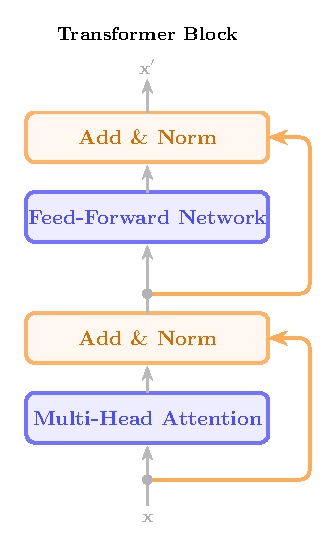
\includegraphics[width=0.3\linewidth, alt={Diagram of a single transformer block. Tokens enter from the bottom and pass through a multi-head self-attention sublayer followed by layer normalization with a residual connection, then through a feed-forward network sublayer followed by a second layer normalization with another residual connection, before exiting at the top.}]{figures/ch3/transformer_block_diagram}
    \caption{A single transformer block. Each block applies multi-head self-attention and a position-wise feed-forward network (FFN), each wrapped in a residual connection and layer normalization. A full transformer is formed by stacking $L$ such blocks.}
    \label{fig:transformer_block}
\end{figure}

Importantly self-attention as defined in \Cref{eqn:attention} is \textit{permutation equivariant}, meaning permuting the rows of $X$ permutes the rows of the output without changing the actual vector representing the items in the set.
In natural language processing this is a problem because word order carries meaning.
This is why Ref.~\cite{Vaswani:2017attention} added \textit{positional encodings} to the input that break permutation symmetry.
However for HEP data permutation equivariance is often a very useful inductive bias~\cite{Komiske:2018cqr}.
Jets and events are composed of unordered sets of particles, where the order of the particles is typically not meaningful\footnote{An exception to this will be covered in the set-to-set unfolding work in \Cref{ch:unfolding}.}.
This means the transformer architecture can be applied to HEP data directly~\cite{Mikuni:2020wpr}, which is why transformers are so widely used in HEP whereas their direct predecessors, RNNs, are not.
